\documentclass[12pt,a4paper]{article}
\usepackage[utf8]{vietnam}
\usepackage{amsmath}
\usepackage{amsfonts}
\usepackage{xcolor}
\usepackage{titlesec}
\usepackage{mdframed}
\usepackage{amssymb}
\usepackage{graphicx}
\usepackage{cases} 
\usepackage{pgfplots}
\pgfplotsset{compat=1.5}
\usepackage{mathrsfs}
\usetikzlibrary{arrows}
\usepackage{fancyhdr}
\usepackage{float}
\usepackage{enumerate}
\usepackage{enumitem}
\pagestyle{fancy}
\pagestyle{empty}
\usepackage[left=2cm,right=2cm,top=2cm,bottom=2cm]{geometry}
\author{Nguyễn Văn Lộc}
\newmdenv[linecolor=black,skipabove=\topsep,skipbelow=\topsep,
leftmargin=-5pt,rightmargin=-5pt,
innerleftmargin=5pt,innerrightmargin=5pt]{mybox}
\begin{document}
\fancyhf{}
\lhead{}
\chead{}
\rhead{}
\cfoot{}
\rfoot{\thepage}
\lfoot{}
\pagestyle{fancy}
\renewcommand{\headrulewidth}{0pt}
\renewcommand{\footrulewidth}{0pt}
\begin{mybox}
\textbf{Họ và tên:} Nguyễn Văn Lộc\\
\textbf{MSSV:} 20120131\\
\textbf{Lớp:} 20CTT1
\end{mybox}
\begin{center}
\fontsize{16}{14}\selectfont
\textbf{Bài tập môn Xác suất thống kê}\\
\textbf{Chương 1: Đại cương về xác suất}
\end{center}
Các bài tập được làm: 1, 2, 3, 4, 6, 7, 8, 9, 10, 11, 13\\
\textbf{Bài 1.} \textit{Một thí sinh đi thi chỉ thuộc $18$ câu trong tổng số $25$ câu hỏi. Đề thi có $3$ câu hỏi. Tính xác suất thí sinh này:}
\begin{enumerate}[label=(\alph*)]
\item \textit{trả lời được $3$ câu.}\\
Không gian mẫu: $n_{\Omega} = C^3_{25}.$\\
Gọi $A$ là biến cố: "thí sinh này trả lời được $3$ câu."\\
Số cách lấy ra $3$ câu hỏi mà thí sinh này thuộc hết là: $n_A = C^3_{18}.$
$$\Rightarrow P\left( A \right) = \frac{{{n_A}}}{{{n_\Omega }}} = \frac{{C_{18}^3}}{{C_{25}^3}} = \frac{{204}}{{575}}.$$
\item \textit{trả lời được ít nhất $2$ câu.}\\
Gọi $B$ là biến cố: "thí sinh này trả lời được ít nhất $2$ câu."\\
Trường hợp 1: thí sinh này trả lời được đúng $2$ câu.\\
Số cách lấy ra $3$ câu hỏi mà thí sinh này trả lời được đúng $2$ câu là: $C^2_{18} C^1_{7}.$\\
Trường hợp 2: thí sinh này trả lời được cả $3$ câu.\\
Số cách lấy ra $3$ câu hỏi mà thí sinh này trả lời được hết là: $C^3_{18}.$\\
$$\Rightarrow n_B = C^2_{18} C^1_{7} + C^3_{18}.$$
$$ \Rightarrow P\left( B \right) = \frac{{{n_B}}}{{{n_\Omega }}} = \frac{{C_{18}^2C_7^1 + C_{18}^3}}{{C_{25}^3}} = \frac{{1887}}{{2300}}.$$
\end{enumerate}
\textbf{Bài 2.} \textit{Có hai lô sản phẩm. Lô thứ nhất có $10$ sản phẩm loại I và $2$ sản phẩm loại II; lô thứ hai có $16$ sản phẩm loại I và $4$ sản phẩm loại II. Từ mỗi lô lấy ngẫu nhiên $1$ sản phẩm, sau đó từ $2$ sản phẩm đã lấy ra lấy ngẫu nhiên $1$ sản phẩm. Tính xác suất sản phẩm lấy ra cuối cùng là loại I.}\\
Không gian mẫu: ${n_\Omega } = C_{12}^1C_{20}^1C_2^1 = 480.$\\
Gọi $A$ là biến cố: "sản phẩm lấy ra cuối cùng là loại I."\\
Trường hợp 1: cả hai sản phẩm lấy ra từ hai lô đều là loại I.\\
Số cách lấy ra thỏa mãn biến cố $A$ là: $C^1_{10} C^1_{16} C^1_{2}.$\\
Trường hợp 2: sản phẩm lấy ra từ lô thứ nhất là loại I, sản phẩm lấy ra từ lô thứ hai là loại II.\\
Số cách lấy ra thỏa mãn biến cố $A$ là: $C^1_{10} C^1_{4} C^1_{1}.$\\
Trường hợp 3: sản phẩm lấy ra từ lô thứ nhất là loại II, sản phẩm lấy ra từ lô thứ hai là loại I.\\
Số cách lấy ra thỏa mãn biến cố $A$ là: $C^1_2 C^1_{16} C^1_1.$\\
Vậy tổng số cách lấy ra thỏa mãn biến cố $A$ là: 
$${n_A} = C_{10}^1C_{16}^1C_2^1 + C_{10}^1C_4^1C_1^1 + C_2^1C_{16}^1C_1^1 = 392.$$
$$ \Rightarrow P\left( A \right) = \frac{{{n_A}}}{{{n_\Omega }}} = \frac{{392}}{{480}} = \frac{{49}}{{60}}.$$
\textbf{Bài 3.} \textit{Một người có ba chỗ ưa thích như nhau để câu cá, xác suất câu được cá ở những chỗ đó lần lượt là $0.6, 0.7, 0.8.$ Người đó vào chỗ thả câu $3$ lần và chỉ câu được $1$ con cá. Tính xác suất con cá câu được ở chỗ thứ nhất.}\\
Gọi $A_i$ là biến cố: "người đó đi câu ở chỗ thứ $i,$ $i = 1, 2, 3$ Ta được: $P \left( {A_i} \right) = \frac{1}{3},$ $i = 1, 2, 3.$\\
Gọi $B$ là biến cố: "câu được $1$ con cá trong $3$ lần đi câu tại địa điểm đã chọn."\\
Ta thấy đây là mô hình các phép thử tuân theo lược đồ Bernoulli. Do đó, áp dụng công thức Bernoulli, ta được:
$$P\left( {\left. B \right|{A_1}} \right) = C_3^1{\left( {0.6} \right)^1}{\left( {0.4} \right)^2} = \frac{{36}}{{125}}.$$
$$P\left( {\left. B \right|{A_2}} \right) = C_3^1{\left( {0.7} \right)^1}{\left( {0.3} \right)^2} = \frac{{189}}{{1000}}.$$
$$P\left( {\left. B \right|{A_3}} \right) = C_3^1{\left( {0.8} \right)^1}{\left( {0.2} \right)^2} = \frac{{12}}{{125}}.$$
$$ \Rightarrow P\left( B \right) = \sum\limits_{i = 1}^3 {P\left( {{A_i}} \right)} P\left( {\left. B \right|{A_i}} \right) = \frac{1}{3}\left( {\frac{{36}}{{125}} + \frac{{189}}{{1000}} + \frac{{12}}{{125}}} \right) = \frac{{191}}{{1000}}.$$
Áp dụng công thức Bayes, ta được:
$$P\left( {\left. {{A_1}} \right|B} \right) = \frac{{P\left( {{A_1}} \right)P\left( {\left. B \right|{A_1}} \right)}}{{P\left( B \right)}} = \frac{{96}}{{191}}.$$
\textbf{Bài 4.} \textit{Trên đoạn thẳng $OA$ ta gieo một cách ngẫu nhiên hai điểm $B, C$ có tọa độ tương ứng là $OB = x, OC = y$ $\left( {y \geqslant x} \right).$ Tìm xác suất sao cho độ dài đoạn $BC$ bé hơn độ dài đoạn $OB.$}\\
\begin{figure}[H]
\begin{center}
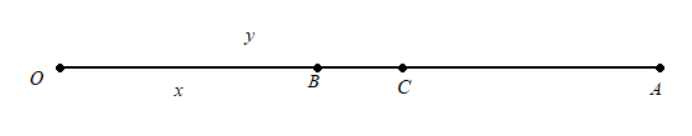
\includegraphics[scale=1]{C1_1}
\end{center}
\end{figure}
Gọi $A$ là biến cố: "độ dài đoạn $BC$ bé hơn độ dài đoạn $OB$".\\
Gọi độ dài đoạn $OA$ là $l.$\\
Độ dài đoạn $BC$ là $BC = y - x.$\\
Độ dài đoạn $BC$ bé hơn độ dài đoạn $OB$ có nghĩa là $y - x < x \Leftrightarrow y < 2x.$\\
Vậy, $y$ thỏa mãn $x \leqslant y < 2x.$
\begin{figure}[H]
\begin{center}
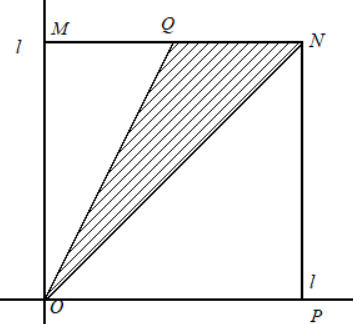
\includegraphics[scale=0.8]{C1_2}
\end{center}
\end{figure}
Miền thỏa mãn đề bài là tam giác $ONQ.$
$$ \Rightarrow P\left( A \right) = \frac{{{S_{ONQ}}}}{{{S_{OMN}}}} = \frac{1}{2}.$$
\textbf{Bài 6.} \textit{Một chuỗi cửa hàng sơn kinh doanh sơn mủ và sơn bán bóng. Dựa trên doanh số bán hàng trong thời gian dài, xác suất để một khách hàng sẽ mua sơn mủ là $0.75.$ Trong số những người mua sơn mủ, $60\%$ cũng mua con lăn. Nhưng chỉ $30\%$ người mua sơn bán bóng mua con lăn. Một người mua được chọn ngẫu nhiên mua một con lăn và một hộp sơn. Tính xác suất hộp sơn đó là sơn mủ.}\\
Gọi $A$ là biến cố: "Người mua đó mua sơn mủ."\\
$B$ là biến cố: "Người mua đó mua sơn bán bóng."\\
$C$ là biến cố: "Người mua đó mua con lăn."\\
Theo đề bài, ta có:
$$P \left( A \right) = 0.75 \Rightarrow P \left( B \right) = 0.25.$$
$$P \left( {\left. C \right|A} \right) = 0.6.$$
$$P \left( {\left. C \right|B} \right) = 0.3.$$
Áp dụng công thức xác suất toàn phần, ta được:
$$P\left( C \right) = P\left( A \right)P\left( {\left. C \right|A} \right) + P\left( B \right)P\left( {\left. C \right|B} \right) = 0.75 \cdot 0.6 + 0.25 \cdot 0.3 = \frac{{21}}{{40}}.$$
Áp dụng công thức Bayes, ta được: 
$$P\left( {\left. A \right|C} \right) = \frac{{P\left( A \right)P\left( {\left. C \right|A} \right)}}{{P\left( C \right)}} = \frac{{0.75 \cdot 0.6}}{{\frac{{21}}{{40}}}} = \frac{6}{7}.$$
\textbf{Bài 7.} \textit{Giả sử khảo sát tình trạng hư hỏng của các điện thoại tại một trung tâm bảo hành điện thoại, người ta nhận thấy $90\%$ số điện thoại bị lỗi phần mềm, $30\%$ số điện thoại bị lỗi phần cứng và tất cả điện thoại ở trung tâm bảo hành này đều bị ít nhất một trong hai lỗi trên. Tính xác suất để một điện thoại bảo hành ở trung tâm này chỉ bị lỗi phần mềm.}\\
Gọi $x$ là số điện thoại tại trung tâm bảo hành.\\
Gọi $A_1$ là số điện thoại bị lỗi phần cứng, $A_2$ là số điện thoại bị lỗi phần mềm.\\
Theo đề bài, ta có:
$$\left\{ \begin{gathered}
  \left| {{A_1}} \right| = 0.9x \hfill \\
  \left| {{A_2}} \right| = 0.3x \hfill \\
  \left| {{A_1} \cup {A_2}} \right| = x \hfill \\ 
\end{gathered}  \right.$$
Theo nguyên lý bù trừ, ta được $\left| A_1 \cap A_2 \right| = 0.2x.$\\
Vậy số điện thoại chỉ bị lỗi phần mềm là $0.7x,$ nghĩa là xác suất điện thoại chỉ bị lỗi phần mềm là $0.7.$\\
\textbf{Bài 8.} \textit{Một dây chuyền lắp ráp nhận các chi tiết từ hai nhà máy khác nhau. Tỉ lệ chi tiết do nhà máy thứ nhất cung cấp là $60\%,$ của nhà máy thứ hai là $40\%.$ Tỉ lệ chính phẩm của nhà máy thứ nhất là $90\%$, của nhà máy thứ hai là $85\%.$ Lấy ngẫu nhiên một chi tiết trên dây chuyền và thấy rằng nó tốt. Tìm xác suất để chi tiết đó do nhà máy thứ nhất sản xuất.} \\
Gọi $A_i$ là biến cố: "chi tiết đó được sản xuất ở nhà máy thứ $i$, $i = 1, 2$."\\
Gọi $B$ là biến cố: "chi tiết đó là chi tiết tốt".\\
$$P\left( {{A_1}} \right) = 0.6,P\left( {{A_2}} \right) = 0.4$$
$$P\left( {\left. B \right|{A_1}} \right) = 0.9$$
$$P\left( {\left. B \right|{A_2}} \right) = 0.85$$
Áp dụng công thức xác suất toàn phần:
$$ \Rightarrow P\left( B \right) = P\left( {{A_1}} \right)P\left( {\left. B \right|{A_1}} \right) + P\left( {{A_2}} \right)P\left( {\left. B \right|{A_2}} \right) = 0.88.$$
Áp dụng công thức Bayes:
$$P\left( {\left. {{A_1}} \right|B} \right) = \frac{{P\left( {{A_1}} \right)P\left( {\left. B \right|{A_1}} \right)}}{{P\left( B \right)}} = \frac{{27}}{{44}}.$$
\textbf{Bài 9.} \textit{Một nhà máy có ba phân xưởng $A, B, C$ tương ứng làm ra $25\%, 35\%, 40\%$ tổng sản phẩm của nhà máy. Giả sử xác suất làm ra một sản phẩm hỏng của các phân xưởng là $0.01, 0.02, 0.025.$ Hãy tính xác suất nhận được một sản phẩm hỏng.}\\
Gọi $A_1, A_2, A_3$ lần lượt là các biến cố: "sản phẩm đó sản xuất tại phân xưởng $A,$" "sản phẩm đó sản xuất tại phân xưởng $B,$" "sản phẩm đó sản xuất tại phân xưởng $C.$"\\
Gọi $B$ là biến cố: "sản phẩm đó là sản phẩm hỏng."\\
$$\left\{ \begin{gathered}
  P\left( {{A_1}} \right) = 0.25 \hfill \\
  P\left( {{A_2}} \right) = 0.35 \hfill \\
  P\left( {{A_3}} \right) = 0.4 \hfill \\ 
\end{gathered}  \right.$$
$$\left\{ \begin{gathered}
  P\left( {\left. B \right|{A_1}} \right) = 0.01 \hfill \\
  P\left( {\left. B \right|{A_2}} \right) = 0.02 \hfill \\
  P\left( {\left. B \right|{A_3}} \right) = 0.025 \hfill \\ 
\end{gathered}  \right.$$
Áp dụng công thức xác suất toàn phần:
$$P\left( B \right) = \sum\limits_{i = 1}^3 {P\left( {{A_i}} \right)P\left( {\left. B \right|{A_i}} \right)}  = \frac{{39}}{{2000}}.$$
\textbf{Bài 10.} \textit{Trong một vùng dân cư, cứ $100$ người thì có $30$ người hút thuốc lá. Biết tỷ lệ người bị viêm họng trong số người hút thuốc lá là $60\%$, trong số người không hút thuốc lá là $30\%$. Khám ngẫu nhiên một người và thấy người đó bị viêm họng. Tìm xác suất để người đó hút thuốc lá. Nếu người đó không bị viêm họng thì xác suất để người đó hút thuốc lá là bao nhiêu?}\\
Gọi $A$ là biến cố: "người đó hút thuốc lá." $\Rightarrow P \left( A \right) = 0.3 \Rightarrow P \left( {\overline{A}} \right) = 0.7.$\\
Gọi $B$ là biến cố: "người đó bị viêm họng."
$$\left\{ \begin{gathered}
  P\left( {\left. B \right|A} \right) = 0.6 \hfill \\
  P\left( {\left. B \right|\overline A } \right) = 0.3 \hfill \\ 
\end{gathered}  \right.$$
Áp dụng công thức xác suất toàn phần:
$$P\left( B \right) = P\left( A \right)P\left( {\left. B \right|A} \right) + P\left( {\bar A} \right)P\left( {\left. B \right|\overline A } \right) = \frac{{39}}{{100}}.$$
Áp dụng công thức Bayes:
$$P\left( {\left. A \right|B} \right) = \frac{{P\left( A \right)P\left( {\left. B \right|A} \right)}}{{P\left( B \right)}} = \frac{6}{{13}}.$$
Nếu không bị viêm họng:
$$P\left( B \right) = \frac{{39}}{{100}} \Rightarrow P\left( {\overline B } \right) = \frac{{61}}{{100}}$$
$$\left\{ \begin{gathered}
  P\left( {\left. B \right|A} \right) = 0.6 \hfill \\
  P\left( {\left. B \right|\overline A } \right) = 0.3 \hfill \\ 
\end{gathered}  \right. \Rightarrow \left\{ \begin{gathered}
  P\left( {\left. {\overline B } \right|A} \right) = 0.4 \hfill \\
  P\left( {\left. {\overline B } \right|\overline A } \right) = 0.7 \hfill \\ 
\end{gathered}  \right.$$
\[P\left( {\left. A \right|\overline B } \right) = \frac{{P\left( A \right)P\left( {\left. {\overline B } \right|A} \right)}}{{P\left( {\overline B } \right)}} = \frac{{12}}{{61}}.\]
\textbf{Bài 11.} \textit{Một thiết bị gồm $3$ cụm chi tiết, mỗi cụm bị hỏng không ảnh hưởng gì đến các cụm khác và chỉ cần một cụm bị hỏng thì thiết bị ngừng hoạt động. Xác suất để cụm thứ nhất bị hỏng trong ngày là $0.1$; cụm thứ hai là $0.05$ và cụm thứ ba là $0.15.$ Tìm xác suất để thiết bị không ngừng hoạt động trong ngày.}\\
Thiết bị không ngừng hoạt động trong ngày khi cả ba cụm đều không bị hỏng trong ngày.\\
Gọi $A$ là biến cố: "thiết bị không ngừng hoạt động trong ngày".\\
Gọi $A_i$ lần lượt là biến cố: "cụm thứ $i$ ngừng hoạt động trong ngày, $i = 1, 2 , 3.$"\\
$$\left\{ \begin{gathered}
  P\left( {{A_1}} \right) = 0.1 \hfill \\
  P\left( {{A_2}} \right) = 0.05 \hfill \\
  P\left( {{A_3}} \right) = 0.15 \hfill \\ 
\end{gathered}  \right. \Rightarrow \left\{ \begin{gathered}
  P\left( {\overline {{A_1}} } \right) = 0.9 \hfill \\
  P\left( {\overline {{A_2}} } \right) = 0.95 \hfill \\
  P\left( {\overline {{A_3}} } \right) = 0.85 \hfill \\ 
\end{gathered}  \right.$$
Do $\overline{A_1}, \overline{A_2},\overline{A_3}$ là ba biến cố độc lập từng đôi nên áp dụng công thức nhân xác suất, ta được:
$$P\left( A \right) = P\left( {\overline {{A_1}} } \right)P\left( {\overline {{A_2}} } \right)P\left( {\overline {{A_3}} } \right) = \frac{{2907}}{{4000}}.$$
\textbf{Bài 13.} \textit{Trong $18$ xạ thủ có $5$ người có khả năng bắn trúng bia với xác suất là $0.8$; $7$ người có khả năng bắn trúng bia với xác suất là $0.7$; $4$ người có khả năng bắn trúng bia với xác suất là $0.6$ và $2$ người có khả năng bắn trúng bia với xác suất là $0.5$. Chọn  ngẫu  nhiên  $1$  xạ  thủ  và  anh  ta  bắn  không  trúng  bia.  Hỏi  anh  ta  có  khả  năng thuộc nhóm nào nhiều hơn?}\\
Gọi $A$ là biến cố: "xạ thủ được chọn bắn không trúng bia".\\
Ta gọi nhóm $5$ người có khả năng bắn trúng bia với xác suất $0.8$ là nhóm $1,$ $7$ người có khả năng bắn trúng bia với xác suất $0.7$ là nhóm $2,$ $4$ người có khả năng bắn trúng bia với xác suất $0.6$ là nhóm $3$ và $2$ người có khả năng bắn trúng bia với xác suất $0.5$ là nhóm $4.$\\
Gọi $A_i$ là biến cố: "xạ thủ được chọn nằm ở nhóm $i,$ $i = 1, 2, 3, 4$".\\
$$\left\{ \begin{gathered}
  P\left( {{A_1}} \right) = \frac{5}{{18}} \hfill \\
  P\left( {{A_2}} \right) = \frac{7}{{18}} \hfill \\
  P\left( {{A_3}} \right) = \frac{2}{9} \hfill \\
  P\left( {{A_4}} \right) = \frac{1}{9} \hfill \\ 
\end{gathered}  \right.$$
$$\left\{ \begin{gathered}
  P\left( {\left. A \right|{A_1}} \right) = \frac{1}{5} \hfill \\
  P\left( {\left. A \right|{A_2}} \right) = \frac{3}{{10}} \hfill \\
  P\left( {\left. A \right|{A_3}} \right) = \frac{2}{5} \hfill \\
  P\left( {\left. A \right|{A_4}} \right) = \frac{1}{2} \hfill \\ 
\end{gathered}  \right.$$
Áp dụng công thức xác suất toàn phần:
$$P\left( A \right) = \sum\limits_{i = 1}^4 {P\left( {{A_i}} \right)} P\left( {\left. A \right|{A_i}} \right) = \frac{{19}}{{60}}.$$
Áp dụng công thức Bayes:
$$P\left( {\left. {{A_1}} \right|A} \right) = \frac{{P\left( {{A_1}} \right)P\left( {\left. A \right|{A_1}} \right)}}{{P\left( A \right)}} = \frac{{10}}{{57}}$$
$$P\left( {\left. {{A_2}} \right|A} \right) = \frac{{P\left( {{A_2}} \right)P\left( {\left. A \right|{A_2}} \right)}}{{P\left( A \right)}} = \frac{7}{{19}}$$
$$P\left( {\left. {{A_3}} \right|A} \right) = \frac{{P\left( {{A_3}} \right)P\left( {\left. A \right|{A_3}} \right)}}{{P\left( A \right)}} = \frac{{16}}{{57}}$$
$$P\left( {\left. {{A_4}} \right|A} \right) = \frac{{P\left( {{A_4}} \right)P\left( {\left. A \right|{A_4}} \right)}}{{P\left( A \right)}} = \frac{{10}}{{57}}$$
Vậy xác suất người đó ở nhóm $2$ là cao nhất.
\end{document}